\section{Phương pháp số trong mô phỏng}\label{sec_2}

Phần này có mục đích giới thiệu một số phương pháp số thường được sử dụng trong mô phỏng vật lý (phương pháp sai phân hữu hạn và phương pháp phần tử hữu hạn). Mục đích của các phương pháp số là xấp xỉ nghiệm của các bài toán điều kiện biên mà trong đó việc giải trực tiếp phương trình vi phân là không thể. Một bài toán điều kiện biên thường được biểu diễn bằng một phương trình đạo hàm riêng và các điều kiện biên đi kèm. Phương trình Poisson 1D trong \cref{eq_PTpoisson_tq} là một ví dụ của bài toán điều kiện biên. Bài toán này có thể giải một cách trực tiếp nếu hàm $f(x)$ là một hàm đơn giản và có thể tích phân. Tuy nhiên trong thực tế, một hàm như vậy không tồn tại nhiều. Vì vậy các phương pháp số đã được phát triển để giải quyết vấn đề này.

\begin{equation}\label{eq_PTpoisson_tq}
    \begin{aligned}
        -\frac{\partial^2u}{\partial x^2} &= f(x) \quad x \in \left(0, L\right) \\
        u\left(0\right) &= u_0 \quad \left(\hbox{điều kiện biên Dirichlet}\right) \\
        \frac{\partial u}{\partial x} \left(L\right) &= u'_L \quad \left(\hbox{điều kiện biên Neumann}\right) \\
    \end{aligned}
\end{equation}

Trong phần còn lại, để đơn giản việc trình bày, chúng ta sẽ chọn $f(x) = x$, $u_0 = 2$ và $u'_L = 1$. Tập xác định của phương trình là $(0, 1)$ (\cref{eq_PTpoisson}). Điều này không làm mất đi tính tổng quát của các phương pháp số, bởi vì việc áp dụng các phương pháp là như nhau cho bất kỳ bài toán điều kiện biên nào.

\begin{equation}\label{eq_PTpoisson}
    \begin{aligned}
        -\frac{\partial^2u}{\partial x^2} &= x \quad x \in \left(0, 1\right) \\
        u\left(0\right) &= 2 \quad \left(\hbox{điều kiện biên Dirichlet}\right) \\
        \frac{\partial u}{\partial x} \left(1\right) &= 1 \quad \left(\hbox{điều kiện biên Neumann}\right) \\
    \end{aligned}
\end{equation}

Với phương trình \cref{eq_PTpoisson}, chúng ta có thể xác định được nghiệm chính xác của nó:

\begin{equation}\label{eq_sol}
    u\left(x\right) = \frac{-x^3 + 9x + 12}{6}
\end{equation}

Các phương pháp số sẽ được áp dụng để giải \cref{eq_PTpoisson} và so sánh với nghiệm chính xác của nó (\cref{eq_sol}).

\subsection{Phương trình vi phân}

Trước khi tìm hiểu các phương pháp số chúng ta cần tìm hiểu một số các biểu diễn các phương trình vi phân, bởi vì với mỗi phương pháp được trình bày sẽ tiếp cận một dạng khác nhau của phương trình.

\subsubsection{Phương trình dạng mạnh}

Phương trình vi phân dạng mạnh là các phương trình mô tả các hiện tương vật lý mà trong đó nghiệm của phương trình thỏa mãn với mọi điểm trong miền xác định. Phương trình Poisson trong \cref{eq_PTpoisson} là một phương trình dạng mạnh. 

\subsubsection{Phương trình dạng yếu}

Phương trình dạng yếu được biểu diễn dưới dạng tích phân của tích phương trình dạng mạnh với một hàm thử trên miền xác định. Ý tưởng là xấp xỉ nghiệm của phương trình dạng mạnh bằng một hàm đơn giản hơn mà việc xác định nó không yêu cầu giải trực tiếp bài toán điều kiện biên. Một trong nhưng phương pháp để biến đổi phương trình dạng mạnh về phương trình dạng yếu đó là phương pháp Ritz-Galerkin.

Chúng ta sẽ bắt đầu bằng việc xấp xỉ nghiệm $u$ của phương trình \cref{eq_PTpoisson} bằng một nghiệm $u^h$. Nghiệm xấp xỉ này sẽ thỏa mãn điều kiện Dirichlet (ie. $u^h(0) = 2$). Vì đây là nghiệm xấp xỉ nên hiển nhiên rằng nghiệm này sẽ không thỏa mãn phương trình vi phân cũng như điều kiện biên Neumann. Vì vậy chúng ta có:

\begin{equation}\label{eq_RR}
    \begin{aligned}
        R_{\Omega} &= -\frac{\partial^2 u^h}{\partial x^2} - x \neq 0 \quad x \in \left(0, 1\right) \\
        R_{\partial\Omega} &= \frac{\partial u^h}{\partial x} \left(1\right) - 1 \neq 0 \\
    \end{aligned}
\end{equation}

Ý tưởng của phương pháp Ritz-Galerkin là nhân các phương trình trong \cref{eq_RR} với một hàm thử $v$ và tích phân trên toàn miền bài toán để tìm nghiệm. Hàm thử này phải thỏa mãn điều kiện Dirichlet \textbf{đồng nhất} $v(0) = 0$. Vì vậy chúng ta có:

\begin{equation}\label{eq_Ritz}
    \begin{aligned}
        &\int\limits_0^1 v R_{\Omega}dx + v(1)R_{\partial\Omega} = 0 \\
        \Rightarrow &\int\limits_0^1 v \left(-\frac{\partial^2 u^h}{\partial x^2} - x\right)dx + v(1)\left(\frac{\partial u^h}{\partial x} \left(1\right) - 1\right) =0
    \end{aligned}
\end{equation}

Sử dụng tích phân từng phần để biến đổi, chúng ta có:

\begin{equation}\label{eq_weakform}
    \int\limits_0^1 \frac{\partial u^h}{\partial x} \frac{\partial v}{\partial x}dx - v(1) - \int\limits_0^1 v x dx =0
\end{equation}

Phương trình \cref{eq_weakform} được gọi là phương trình dạng yếu. Theo nguyen ly Bubnov-Galerkin, ham thu se duoc chon sao cho no co cung ham noi suy doi voi $u^h$. Viec xac dinh cac ham noi suy se duoc trinh bay trong phuong phap phan tu huu han.

\subsection{Phương pháp số}

\subsubsection{Phương pháp sai phân hữu hạn}

Phương pháp sai phân hữu hạn là phương pháp xấp xỉ nghiệm trực tiếp từ phương trình dạng mạnh. Ý tưởng của phương pháp này là sử dụng chuỗi Taylor để xấp xỉ các đạo hàm và thay vào phương trình vi phân.

\begin{equation}\label{eq_taylor}
    \begin{aligned}
        f(x+h) &=f(x)+f^{\prime}(x) h+\frac{f^{\prime \prime}(x)}{2!} h^2+\frac{f^{\prime \prime \prime}(x)}{3!} h^3+\frac{f^{(4)}\left(\xi_1\right)}{4!} h^4 + \dots\\
        f(x-h) &=f(x)-f^{\prime}(x) h+\frac{f^{\prime \prime}(x)}{2!} h^2-\frac{f^{\prime \prime \prime}(x)}{3!} h^3+\frac{f^{(4)}\left(\xi_2\right)}{4!} h^4 + \dots
\end{aligned}
\end{equation}

Từ đây, chúng ta có các cách để xấp xỉ đạo hàm bậc nhất như sau:

\begin{equation}\label{eq_bac1}
    \begin{aligned}
        f^{\prime}(x) &\approx \frac{f(x+h) - f(x)}{h} \quad \hbox{sai phân tiến} \\
        f^{\prime}(x) &\approx \frac{f(x) - f(x-h)}{h} \quad \hbox{sai phân lùi} \\
        f^{\prime}(x) &\approx \frac{f(x+h) - f(x-h)}{2h} \quad \hbox{sai phân trung tâm} \\
    \end{aligned}
\end{equation}

Xấp xỉ đạo hàm bậc 2 cũng được suy ra như sau:

\begin{equation}\label{eq_bac2}
    f^{\prime \prime}(x) \approx \frac{f(x+h) -2f(x) + f(x-h)}{h^2}
\end{equation}

Ap dung cho bai toan tren, ta chia mien tich phan thanh $N=3$ diem luoi voi toa do lan luot la $x_1 = 0$, $x_2 = 0.5$, $x_3=1$ ($h=1/(N-1)$). Ap dung xap xi Taylor bac 2 cho nut 2:

\begin{equation}
    - \frac{u_1 - 2u_2 +u_3}{h^2} = x_2
\end{equation}

Dieu kien bien Neumann duoc xac dinh nhu sau:

\begin{equation}
    \frac{u_3 -u_2}{h} = 1
\end{equation}

Ket hop cac phuong trinh va voi dieu kien bien Dirichlet, ta co he sau:

\begin{equation}
    \begin{bmatrix}
        1 & 0 & 0 \\ 1/h^2 & -2/h^2 & 1/h^2 \\ 0 & -1/h^2 & 1/h^2 
    \end{bmatrix}\begin{bmatrix}
        u_1 \\ u_2 \\ u_3 
    \end{bmatrix} = \begin{bmatrix}
        2 \\ x_2 \\ 1
    \end{bmatrix}
\end{equation}

Giai he phuong trinh tren ta thu duoc gia tri tai cac nut. Do chinh xac cua phuong phap nay phu thuoc vao do min cua luoi da chia. Voi 3 nut thi ket qua co sai so kha lon so voi nghiem chinh xac. Tuy nhien neu tang dan so luong nut len thi ta se thu duoc ket qua cang gan voi nghiem chinh xac \cref{fig_SPHHresults}

\begin{figure}[htbp]
    \centering
    \begin{subfigure}[b]{0.3\linewidth}
        \centering
        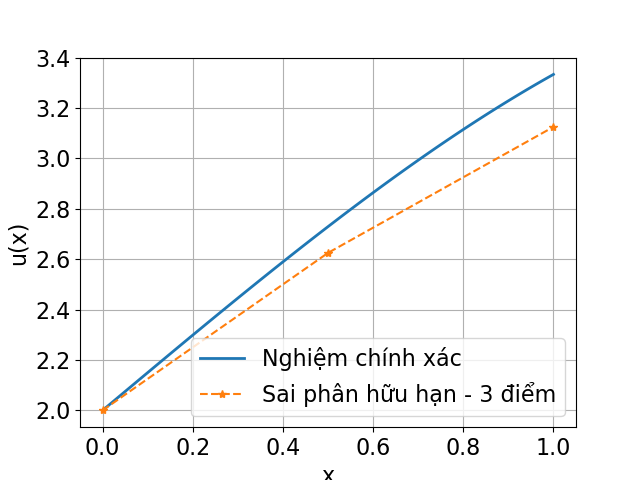
\includegraphics[width=\linewidth]{Tuan6/figure/SPHH_3p.png}
        \caption{3 nút}
        \label{fig:SPHH_3p}
    \end{subfigure}\hfill
    \begin{subfigure}[b]{0.3\linewidth}
        \centering
        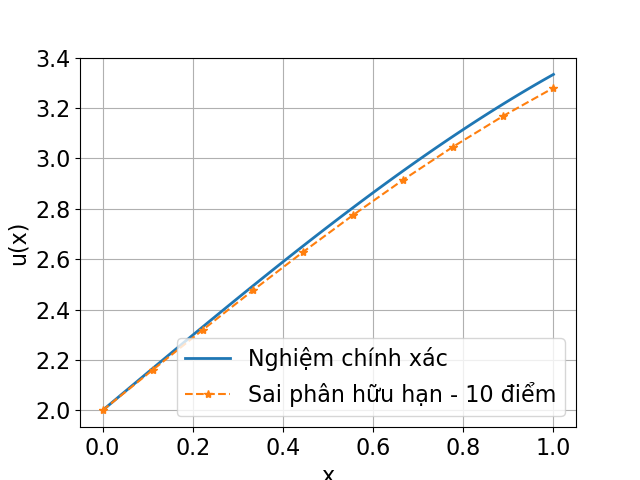
\includegraphics[width=\linewidth]{Tuan6/figure/SPHH_10p.png}
        \caption{10 nút}
        \label{fig:SPHH_10p}
    \end{subfigure}\hfill
    \begin{subfigure}[b]{0.3\linewidth}
        \centering
        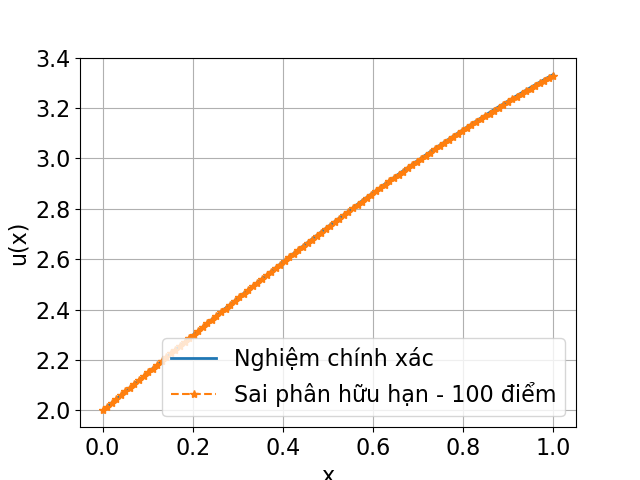
\includegraphics[width=\linewidth]{Tuan6/figure/SPHH_100p.png}
        \caption{100 nút}
        \label{fig:SPHH_100p}
    \end{subfigure}
    \caption{Nghiệm của PT Poisson bằng phương pháp sai phân hữu hạn với (a) 3 nút, (b) 10 nút, (c) 100 nút.}
    \label{fig_SPHHresults}
\end{figure}


\subsubsection{Phương pháp phần tử hữu hạn}

Ý tưởng của phương pháp này là chia miền xác định thành các miền con $\Omega_e$ không giao nhau gọi là các phần tử (chia lưới). Các phần tử liên kết với nhau tại các nút đặt tại các đỉnh của phần tử. Đối với miền 1D thì phần tử là các đoạn thẳng có các nút ở 2 đầu. Miền 2D thì phần tử là các đa giác (thường là tam giác hoặc tứ giác với nút đặt tại các đỉnh). 

Xét bài toán 1D, miền xác định được chia thành m miền con, số nút tương ứng là $n = m+1$,mỗi nút có tọa độ $x_i$, mỗi phần tử giới hạn bởi $\Omega_e = [x_i, x_{i+1}]$. Mỗi nút liên kết với 1 hàm dạng (hàm nội suy) $N_i(x)$. Hàm dạng thường là các hàm đa thức thỏa mãn tính chất $N_i(x_i) = 1$ và $N_i(x_j) = 0$ với $j \neq i$.

Nghiệm xấp xỉ theo phương pháp phần tử hữu hạn lúc này sẽ được biểu diễn bởi 

\begin{equation}\label{eq_interpolation}
    u^h(x) = \sum\limits_{i=1}^n N_i(x) u_i = \underbrace{\begin{bmatrix}
        N_1(x) \dots N_n(x)
    \end{bmatrix}}_{{\bf N}(x)} \underbrace{\begin{bmatrix}
        u_1 \\ \vdots \\ u_n 
    \end{bmatrix}}_{\bf u}
\end{equation}

Vector ${\bf u}$ chứa các phần tử là giá trị của $u^h(x)$ tại các nút và được gọi là bậc tự do của bài toán. Chia lưới càng mịn thì sẽ dẫn đến số lượng bậc tự do sẽ tăng lên càng nhiều.

Ham thu $v$ cung duoc bieu dien bang cach tuong tu: 

\begin{equation}\label{eq_interpolation_test}
    v(x) = \sum\limits_{i=1}^n N_i(x) v_i = {{\bf N}(x)}{\bf v}
\end{equation}

Thay cac xap xi nay vao phuong trinh dang yeu \cref{eq_weakform}, ta co:

\begin{equation}
    {\bf v}^T\left(\int\limits_0^1\left(\frac{\partial{\bf N}}{\partial x}\right)^T\frac{\partial{\bf N}}{\partial x} dx\right){\bf u} - {\bf v}^T[{\bf N}(1)]^T - {\bf v}^T\int\limits_0^1 [{\bf N}(x)]^Tx dx = 0
\end{equation}

Rut gon phuong trinh nay ta co:

\begin{equation}\label{eq_matrixform}
    \underbrace{\left(\int\limits_0^1\left(\frac{\partial{\bf N}}{\partial x}\right)^T\frac{\partial{\bf N}}{\partial x} dx\right)}_{\bf K}{\bf u} = \underbrace{[{\bf N}(1)]^T + \int\limits_0^1 [{\bf N}(x)]^Tx dx}_{\bf F} 
\end{equation}

Giai PT \cref{eq_matrixform}, chung ta se tim duoc gia tri cua vector bac tu do. ${\bf u} = {\bf K}^{-1}{\bf F}$

Xet voi bai toan 1D. Cac phan tu la cac doan thang co 2 nut, voi ham dang duoc viet nhu sau (\cref{eq_shape1D,fig_shape_func}):

\begin{equation}\label{eq_shape1D}
    \begin{aligned}
        N_1(x) &= \frac{1}{x_2-x_1}\left(x_2-x\right) \\
        N_2(x) &= \frac{1}{x_2-x_1}\left(x-x_1\right) \\
    \end{aligned}
\end{equation}

\begin{figure}[htbp]
    \centering
    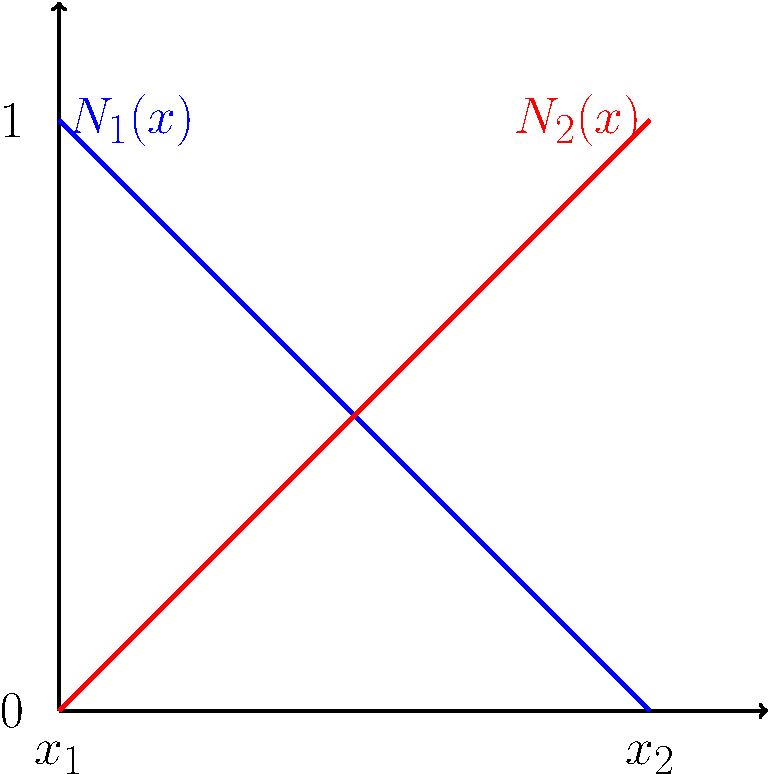
\includegraphics[width=0.3\linewidth]{Tuan6/figure/shape_func.pdf}
    \caption{Ham noi suy 1D}
    \label{fig_shape_func}
\end{figure}

Chung ta de thay rang cac ham dang la nhu nhau doi voi cac phan tu co hinh dang giong nhau. Day la diem dac biet cua phuong phap phan tu huu han. Gia su mien tich phan duoc chia thanh 100 phan tu voi 101 nut thi chung ta khong can phai tich phan de tim tung phan tu trong ma tran ${\bf K}$, ma thay vao do chung ta xac dinh ma tran ${\bf K}_e$ cua tung phan tu va \textbf{lap rap} chung vao ma tran ${\bf K}$.

Quay lai voi phuong trinh poisson 1D, chung ta xe bat dau bang viec xac dinh ma tran ${\bf K}_e$ cua 1 phan tu gioi han boi $[x_1, x_2]$. Dat $L_e = x_2 -x_1$, ta co:

\begin{equation}\label{eq_Ke}
    \begin{aligned}
        {\bf K}_e &= \int\limits_{x_1}^{x_2}\left(\frac{\partial{\bf N}}{\partial x}\right)^T\frac{\partial{\bf N}}{\partial x} dx \\
        & =\int\limits_{x_1}^{x_2}\begin{bmatrix}
            \frac{\partial N_1}{\partial x} \\ \frac{\partial N_2}{\partial x}
        \end{bmatrix}\begin{bmatrix}
            \frac{\partial N_1}{\partial x} &\frac{\partial N_2}{\partial x}
        \end{bmatrix}dx = \int\limits_{x_1}^{x_2}\begin{bmatrix}
            \frac{-1}{L_e} \\ \frac{1}{L_e}
        \end{bmatrix}\begin{bmatrix}
            \frac{-1}{L_e}& \frac{1}{L_e}
        \end{bmatrix}dx \\
        &= \int\limits_{x_1}^{x_2}\begin{bmatrix}
            \frac{1}{L_e^2} & \frac{-1}{L_e^2} \\
            \frac{-1}{L_e^2} & \frac{1}{L_e^2}
        \end{bmatrix}dx = \begin{bmatrix}
            \frac{1}{L_e} & \frac{-1}{L_e} \\
            \frac{-1}{L_e} & \frac{1}{L_e}
        \end{bmatrix} = \begin{bmatrix}
            K_{11} & K_{12} \\
            K_{21} & K_{22}
        \end{bmatrix}
    \end{aligned}
\end{equation}

So hang $ \int\limits_0^1 [{\bf N}(x)]^Tx dx$ cung duoc tinh bang cach tuong tu:

\begin{equation}
    \begin{aligned}
        \int\limits_{x_1}^{x_2} [{\bf N}(x)]^Tx dx &= \int\limits_{x_1}^{x_2} \begin{bmatrix}
            N_1 \\ N_2
        \end{bmatrix}x dx \\
        & = \int\limits_{x_1}^{x_2}\begin{bmatrix}
            \frac{x_2-x}{L_e} \\ \frac{x-x_1}{L_e}
        \end{bmatrix}x dx = \begin{bmatrix}
            \frac{x_2^3-3x_2x_1^2+2x_1^3}{6L_e} \\ \frac{2x_2^3-3x_1x_2^2+x_1^3}{6L_e}
        \end{bmatrix} = \begin{bmatrix}
            F_1 \\ F_2
        \end{bmatrix}
    \end{aligned}
\end{equation}

Chung ta da co ma tran ${\bf K}_e$ cho moi phan tu. Gia su mien tich phan cua chung ta duoc chia thanh 2 phan tu bang nhau $e1$ va $e2$. Toa do cua cac nut lan luot la $x_1 = 0, x_2 = 0.5, x_3 = 1$. Luc nay vector bac tu do se la ${\bf u} = [u_1 \; u_2 \; u_3]^T$. Trong do nut 2 se la diem ket noi giua 2 phan tu, vi vay $u_2 = u_2^{e1} + u_2^{e2}$. Ta co:

\begin{equation}
    {\bf K}_{e1}{\bf u}_{e1} = \begin{bmatrix}
        K_{11}^{e1} & K_{12}^{e1} \\
        K_{21}^{e1} & K_{22}^{e1}
    \end{bmatrix}\begin{bmatrix}
        u_1 \\ u_2^{e1}
    \end{bmatrix} \quad \hbox{va} \quad {\bf K}_{e2}{\bf u}_{e2} = \begin{bmatrix}
        K_{22}^{e2} & K_{23}^{e2} \\
        K_{32}^{e2} & K_{33}^{e2}
    \end{bmatrix}\begin{bmatrix}
        u_2^{e2} \\ u_3
    \end{bmatrix}
\end{equation}

Ket hop 2 PT tren voi $u_2 = u_2^{e1} + u_2^{e2}$, ta co:

\begin{equation}
    {\bf K}{\bf u} = \begin{bmatrix}
        K_{11}^{e1} & K_{12}^{e1} & 0\\
        K_{21}^{e1} & K_{22}^{e1}+K_{22}^{e2} & K_{23}^{e2} \\
        0 & K_{32}^{e2} & K_{33}^{e2}
    \end{bmatrix}\begin{bmatrix}
        u_1 \\ u_2 \\ u_3
    \end{bmatrix}
\end{equation}

Lam tuong tu voi tich phan $ \int\limits_0^1 [{\bf N}(x)]^Tx dx$, ta co:

\begin{equation}
    \int\limits_0^1 [{\bf N}(x)]^Tx dx = \begin{bmatrix}
        F_1^{e1} \\ F_2^{e1}+F_2^{e2} \\ F_3^{e2}
    \end{bmatrix}
\end{equation}

Thay vao phuong trinh \cref{eq_matrixform}, ta co:

\begin{equation}
    \begin{bmatrix}
        K_{11}^{e1} & K_{12}^{e1} & 0\\
        K_{21}^{e1} & K_{22}^{e1}+K_{22}^{e2} & K_{23}^{e2} \\
        0 & K_{32}^{e2} & K_{33}^{e2}
    \end{bmatrix}\begin{bmatrix}
        u_1 \\ u_2 \\ u_3
    \end{bmatrix} = \begin{bmatrix}
        0 \\ 0 \\ 1
    \end{bmatrix} + \begin{bmatrix}
        F_1^{e1} \\ F_2^{e1}+F_2^{e2} \\ F_3^{e2}
    \end{bmatrix}
\end{equation}

Thay so vao PT tren:

\begin{equation}
    \begin{bmatrix}
        2 & -2 & 0\\
        -2 & 2+2 & -2 \\
        0 & -2 & 2
    \end{bmatrix}\begin{bmatrix}
        u_1 \\ u_2 \\ u_3
    \end{bmatrix} = \begin{bmatrix}
        1/24 \\ 1/12 + 1/6 \\ 5/24 + 1
    \end{bmatrix}
\end{equation}

Phuong trinh tuyen tinh nay van chua the giai duoc vi dinh thuc cua ma tran ${\bf K}$ la bang 0. De giai duoc phuong trinh nay can phai ket hop voi dieu kien bien Dirichlet ban dau. Ta co $u(0) = 2$. Thay vao phuong trinh tren va luot bo hang dau, ta co:

\begin{equation}
    \begin{bmatrix}
        -2 & 4 & -2 \\
        0 & -2 & 2
    \end{bmatrix}\begin{bmatrix}
        2 \\ u_2 \\ u_3
    \end{bmatrix} = \begin{bmatrix}
        1/4 \\ 29/24
    \end{bmatrix} \Leftrightarrow \begin{bmatrix}
        4 & -2 \\
        -2 & 2
    \end{bmatrix}\begin{bmatrix}
        u_2 \\ u_3
    \end{bmatrix} = \begin{bmatrix}
        1/4 \\ 29/24
    \end{bmatrix} - 2\begin{bmatrix}
        -2 \\ 0
    \end{bmatrix}
\end{equation}

Giai phuong trinh tim $u_2$ va $u_3$. Chung ta co:
\begin{equation}
    {\bf u} = \begin{bmatrix}
        2 \\ 131/48 \\ 10/3
    \end{bmatrix}
\end{equation}

Thay doi so phan tu chung ta thu duoc ket qua duoi day \cref{fig_PTHHresults}:

\begin{figure}[htbp]
    \centering
    \begin{subfigure}[b]{0.3\linewidth}
        \centering
        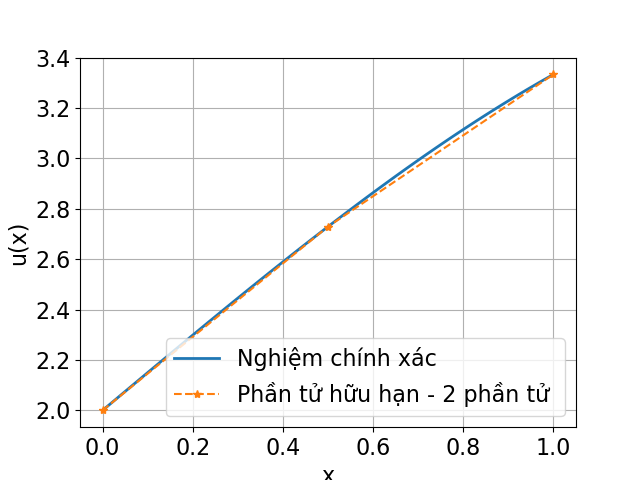
\includegraphics[width=\linewidth]{Tuan6/figure/PTHH_2el.png}
        \caption{}
        \label{fig:PTHH_2el}
    \end{subfigure}\hfill
    \begin{subfigure}[b]{0.3\linewidth}
        \centering
        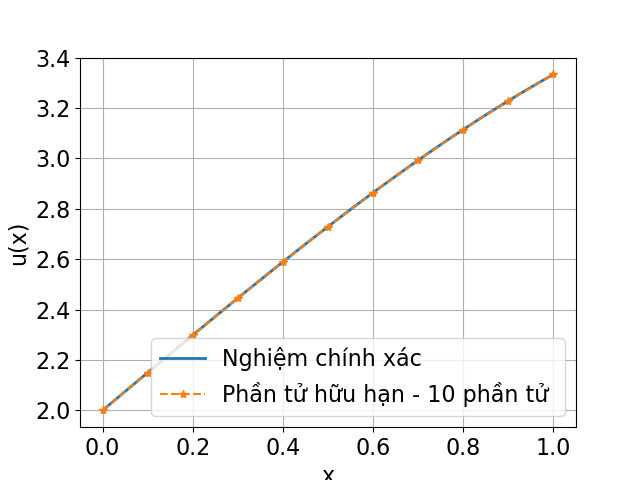
\includegraphics[width=\linewidth]{Tuan6/figure/PTHH_10el.png}
        \caption{}
        \label{fig:PTHH_10el}
    \end{subfigure}\hfill
    \begin{subfigure}[b]{0.3\linewidth}
        \centering
        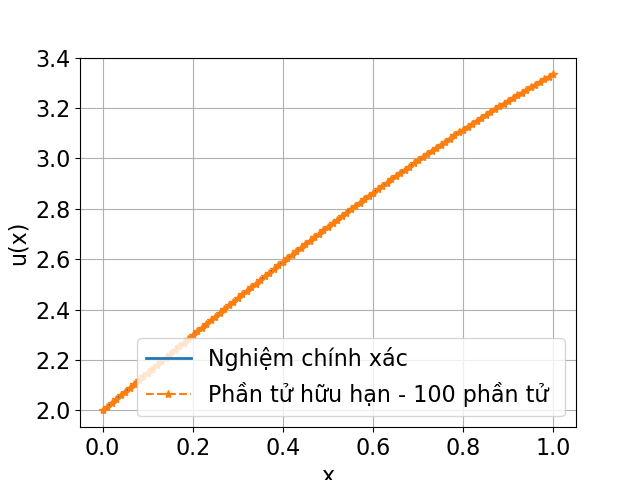
\includegraphics[width=\linewidth]{Tuan6/figure/PTHH_100el.png}
        \caption{}
        \label{fig:PTHH_100el}
    \end{subfigure}
    \caption{Nghiệm của PT Poisson bằng phương pháp phần tử hữu hạn: (a) 2 phần tử, (b) 10 phần tử, (c) 100 phần tử.}
    \label{fig_PTHHresults}
\end{figure}
\textbf{\textcolor{red}{Cau hoi: Moi nguoi co nhan xet gi ve 2 PP da duoc trinh bay? (uu diem, nhuoc diem, gioi han, etc.)}}

\subsection{Tich phan theo thoi gian}

Phuong trinh Poisson khao sat ben tren la mot phuong trinh khong phu thuoc vao thoi gian. Cau hoi dat ra la neu voi nhung bai toan co phu thuoc vao thoi gian thi cac phuong phap ben tren co giai duoc khong. Cau tra loi la hoan toan co the. Y tuong chung la mien tich phan thoi gian se duoc chia thanh cac buoc thoi gian $t_0, t_1, t_2, t_3, t_4, \dots, t_n$ voi buoc thoi gian la $\Delta t = (t_n-t_0)/n$

Voi phuong phap sai phan huu han thi chung ta tiep tuc xap xi dao ham theo thoi gian cua ham so bang phuong phap tuong tu. Luc nay ngoai viec giai phuong trinh tuyen tinh de tim gia tri tai tung nut thi chung ta can ap dung cac phuong phap lap de tim bien thien cua cac nut theo thoi gian (VD: phuong phap Crank–Nicolson). Phan nay se khong duoc gioi thieu trong nay, neu can moi nguoi co the tu tim hieu them

Doi voi phuong phap phan tu huu han thi ngoai ma tran ${\bf K}_e$ ben tren, mot ma tran ${\bf M}_e$ tuong ung cho moi phan tu se xuat hien. Phuong trinh phan tu huu han cho mot phuong trinh dao ham rieng co phu thuoc thoi gian bat ky co dang tong quat nhu sau.

\begin{equation}\label{eq_PTHH_general}
    {\bf M}\ddot{\bf u} + {\bf C}\dot{\bf u} + {\bf K}{\bf u} = {\bf F}
\end{equation}

Chung ta co the thay rang phuong trinh nay co dang tuong tu voi phuong trinh ma tran cua bai toan dao dong dieu hoa 2 bac tu do phia tren !!!

Mot trong nhung phuong phap thong dung de giai quyet bai toan nay la phuong phap Runge-Kutta. Day la mot phuong phap vong lap dung de giai phuong trinh dao ham bac 1. 

\begin{equation}
    \frac{d {\bf u}}{d t}={\bf f}(t,{\bf u}) ,\quad {\bf u}\left(t_0\right)={\bf u}_0
\end{equation}

Tren python phuong phap nay co san trong thu vien \textbf{scipy.integrate}. De su dung chung ta dung ham \textbf{odeint}. Tuy nhien mot diem can luu y la phuong phap nay giai phuong trinh vi phan bac 1 theo thoi gian. Con phuong trinh cua chung ta la phuong trinh vi phan bac 2 theo thoi gian. De giai quyet van de nay chung ta can thuc hien mot thao tac doi bien. 

Dau tien chung ta dat ${\bf u}_1 = {\bf u}$ va ${\bf u}_2 = \dot{\bf u}$. Do do ta co: $\dot{\bf u}_1 = \dot{\bf u}$ va $\dot{\bf u}_2 = \ddot{\bf u}$.

Thay cac bien moi vao phuong trinh ta co:

\begin{equation}
    \begin{aligned}
    &\begin{cases}
        \dot{\bf u}_1 &= {\bf u}_2 \\
        \dot{\bf u}_2 &= {\bf M}^{-1}\left(-{\bf K}{\bf u}_1-{\bf C}{\bf u}_2 + {\bf F}\right)
    \end{cases} \\
    \Rightarrow &\begin{bmatrix}
        \dot{\bf u}_1 \\ \dot{\bf u}_2
    \end{bmatrix} = \begin{bmatrix}
        {\bf O} & {\bf I} \\
        -{\bf M}^{-1}{\bf K} & -{\bf M}^{-1}{\bf C}
    \end{bmatrix}\begin{bmatrix}
        {\bf u}_1 \\ {\bf u}_2
    \end{bmatrix} + \begin{bmatrix}
        {\bf O} \\ {\bf M}^{-1}{\bf F}
    \end{bmatrix} \\
    \Leftrightarrow & \dot{\bf U} = {\bf A} {\bf U} + {\bf B}
    \end{aligned}
\end{equation}

Tu day chung ta co the ap dung ham \textbf{odeint} de giai phuong trinh tim gia tri cua ${\bf U}$.

Phuong phap nay la phuong phap duoc su dung rong rai nhat hien nay de tinh toan so cac tich phan. Tuy nhien khi ap dung de giai phuong trinh phan tu huu han \cref{eq_PTHH_general} thi no co mot nhuoc diem. Do la viec ap dung PP Runge-Kutta se lam tang gap doi so bac tu do cua phuong trinh. Trong phuong phap phan tu huu han, so luong bac tu do phu thuoc vao so phan tu va co the len den hang nghin hoac hang trieu. Vi vay Runge-Kutta khong phai la mot phuong phap toi uu trong truong hop nay.

Trong phan tu huu han, phuong phap tich phan so thuong duoc su dung hon do la phuong phap Newmark. Phuong phap Newmark xap xi cac dao ham bac nhat va bac 2 nhu sau:

\begin{equation}\label{eq_newmark}
    \begin{aligned}
    \dot{\bf u}_{n+1} &\approx \dot{\bf u}_n+(1-\gamma) \Delta t \ddot{\bf u}_n+\gamma \Delta t \ddot{\bf u}_{n+1}\\
    {\bf u}_{n+1} &\approx {\bf u}_n+\Delta t \dot{\bf u}_n+\left(\frac{1}{2}-\beta\right)(\Delta t)^2 \ddot{\bf u}_n+\beta(\Delta t)^2 \ddot{\bf u}_{n+1}
\end{aligned}
\end{equation}

$(\gamma, \beta)$ la cac tham so Newmark. Mot vai gia tri thuong duoc su dung la $(1/2, 1/4)$, $(1/2, 1/6)$, $(1/2, 0)$.

Thay PT \cref{eq_newmark} vao \cref{eq_PTHH_general}, ta co:

\begin{equation}
    \begin{aligned}
    \ddot{\bf u}_{n+1}={\bf S}^{-1}\left[{\bf F}_{n+1}-[{\bf C}\left(\dot{\bf u}_n\right.\right. & \left.+(1-\gamma) \Delta t \ddot{\bf u}_n\right) \\
& \left.-{\bf K}\left({\bf u}_n+\Delta t \dot{\bf u}_n+\left(\frac{1}{2}-\beta\right)(\Delta t)^2 \ddot{\bf u}_n\right)\right]
\end{aligned}
\end{equation}

Voi ${\bf S} = {\bf M} + {\bf C}\gamma\Delta t + {\bf K}\beta(\Delta t)^2$.

O thoi diem ban dau $t_0=0$, ta da biet ${\bf u}_0$ va $\dot{\bf u}_0$. Ta tinh duoc $\ddot{\bf u}_0$ nho vao phuong trinh \cref{eq_PTHH_general}. Tu do ta tim duoc $\ddot{\bf u}_1$. ${\bf u}_1$ va $\dot{\bf u}_1$ duoc suy ra tu \cref{eq_newmark}. Tiep tuc nhu vay ta se tim duoc tat cac cac gia tri tai cai thoi diem tiep theo.